% ! Tex program = xelatex
\documentclass{article}
\PassOptionsToPackage{quiet}{fontspec}% (or try silent)

% 中文
\usepackage[UTF8]{ctex}


% For more choices
% %! Tex program = xelatex
% \documentclass{article}
%中文
%\usepackage[UTF8]{ctex}
%数学公式
\usepackage{amsmath,amssymb}
%\usepackage{ntheorem}
% \usepackage[framemethod=TikZ]{mdframed}
\usepackage{amsthm}
%边界
\usepackage[letterpaper,top=3cm,bottom=3cm,left=2cm,right=2cm,marginparwidth=1.75cm]{geometry}%table package
%Table
\usepackage{multirow,booktabs}
\usepackage{makecell}
%字体颜色
\usepackage{color}
\usepackage[dvipsnames]{xcolor}  % 更全的色系
%代码
\usepackage[OT1]{fontenc}
% MATLAB 代码风格
% \usepackage[framed,numbered,autolinebreaks,useliterate]{/Users/anye_zhenhaoyu/Desktop/Latex/mcode}
\usepackage{listings}
\usepackage{algorithm}
\usepackage{algorithmic}
\usepackage{pythonhighlight} % Python
%插图
\usepackage{graphicx}
%改变item格式
\usepackage{enumerate}
%物理
\usepackage{physics}
%extra arrows
\usepackage{extarrows}
% caption(居中指令)
\usepackage[justification=centering]{caption}
% \usepackage{caption}
% htpb
\usepackage{stfloats}
% pdf 拼接
\usepackage{pdfpages}
% 超链接url
\usepackage{url}
% \usepackage{tikz}
\usepackage{pgfplots}
\pgfplotsset{compat=newest}
\usepackage[colorlinks=true, allcolors=blue]{hyperref}
\usepackage{setspace}

% --------------definations-------------- %
\def\*#1{\boldsymbol{#1}}
\def\+#1{\mathcal{#1}} 
\def\-#1{\bar{#1}}
% Domains
\def\RR{\mathbb{R}}
\def\CC{\mathbb{C}}
\def\NN{\mathbb{N}}
\def\ZZ{\mathbb{Z}}
% Newcommand
\newcommand{\inner}[2]{\langle #1,#2\rangle} 
\newcommand{\numP}{\#\mathbf{P}} 
\renewcommand{\P}{\mathbf{P}}
\newcommand{\Var}[2][]{\mathbf{Var}_{#1}\left[#2\right]}
\newcommand{\E}[2][]{\mathbf{E}_{#1}\left[#2\right]}
\renewcommand{\emptyset}{\varnothing}
\newcommand{\ol}{\overline}
\newcommand{\argmin}{\mathop{\arg\min}}
\newcommand{\argmax}{\mathop{\arg\max}}
\renewcommand{\abs}[1]{\qty|#1|}
\newcommand{\defeq}{\triangleq} % triangle over =
\def\deq{\xlongequal{def}} % 'def' over =
\def\LHS{\text{LHS}}
\def\RHS{\text{RHS}}
\def\angbr#1{\langle#1\rangle} % <x>

\def\Esolve{\textcolor{blue}{Solve: }}
\def\Eproof{\textcolor{blue}{Proof: }}
\def\case#1{\textcolor{blue}{Case \uppercase\expandafter{\romannumeral#1}: }}

\newtheorem{lemma}{Lemma}
\newtheorem{thm}{Theorem}
\newtheorem{defi}{Definition}
\newtheorem{prp}{Proposition}
\newenvironment{md}{\begin{mdframed}}{\end{mdframed}}

\date{\today}
\usepackage{fancyhdr}
\pagestyle{fancy}
\fancyhead[L]{\slshape{Haoyu Zhen}}
\fancyhead[R]{{\today}}

% \begin{document}
% \title{<++>}
\author{Haoyu Zhen}
% \maketitle
\setlength{\parindent}{0pt}
\setstretch{1.2}
% \end{document}


% % theorems
\usepackage{thmtools}
\usepackage{thm-restate}
\usepackage[framemethod=TikZ]{mdframed}
\mdfsetup{skipabove=1em,skipbelow=0em, innertopmargin=12pt, innerbottommargin=8pt}

\theoremstyle{definition}

\declaretheoremstyle[headfont=\bfseries\sffamily, bodyfont=\normalfont,
	mdframed={
		nobreak,
		backgroundcolor=brown!14,
		topline=false,
		rightline=false,
		leftline=true,
		bottomline=false,
		linewidth=2pt,
		linecolor=brown!180,
	}
]{thmbrownbox}

\declaretheoremstyle[headfont=\bfseries\sffamily, bodyfont=\normalfont,
	mdframed={
		nobreak,
		backgroundcolor=Blue!4,
		topline=false,
		rightline=false,
		leftline=true,
		bottomline=false,
		linewidth=2pt,
		linecolor=NavyBlue!120,
	}
]{thmbluebox}

\declaretheoremstyle[headfont=\bfseries\sffamily, bodyfont=\normalfont,
	mdframed={
		nobreak,
		backgroundcolor=Green!5,
		topline=false,
		rightline=false,
		leftline=true,
		bottomline=false,
		linewidth=2pt,
		linecolor=OliveGreen!120,
	}
]{thmgreenbox}

\declaretheoremstyle[headfont=\bfseries\sffamily, bodyfont=\normalfont,
	mdframed={
		nobreak,
		topline=false,
		rightline=false,
		leftline=true,
		bottomline=false,
		linewidth=2pt,
		linecolor=OliveGreen!120,
	}
]{thmgreenline}

\declaretheoremstyle[headfont=\bfseries\sffamily, bodyfont=\normalfont,
	mdframed={
		nobreak,
		topline=false,
		rightline=false,
		leftline=true,
		bottomline=false,
		linewidth=2pt,
		linecolor=NavyBlue!70,
	}
]{thmblueline}

\declaretheorem[numberwithin=section, style=thmbrownbox, name={\color{Brown}Definition}]{defi}
\declaretheorem[numberwithin=section, style=thmgreenbox, name={\color{OliveGreen}Law}]{law}
\declaretheorem[numberwithin=section, style=thmbluebox, name={\color{Blue}Corollary}]{cor}
\declaretheorem[numberwithin=section, style=thmgreenline, name={\color{OliveGreen}Property}]{prt}
\declaretheorem[numberwithin=section, style=thmbluebox, name={\color{Blue}Proposition}]{prp}
\declaretheorem[numberwithin=section, style=thmbluebox, name={\color{Blue}Theorem}]{thm}
\declaretheorem[numberwithin=section, style=thmbluebox, name={\color{Blue}Lemma}]{lemma}
\declaretheorem[numberwithin=section, style=thmbrownbox,  name={\color{Brown}Example}]{eg}
\declaretheorem[numberwithin=section, style=thmgreenline, name={\color{OliveGreen}Remark}]{remark}
\declaretheorem[numbered=no,style=thmblueline, name={\color{NavyBlue!70}Proof},qed=$\square$]{prf}
\numberwithin{equation}{section}


% %! Tex program = xelatex
% \documentclass{article}
%中文
%\usepackage[UTF8]{ctex}
%数学公式
\usepackage{amsmath,amssymb}
%\usepackage{ntheorem}
% \usepackage[framemethod=TikZ]{mdframed}
\usepackage{amsthm}
%边界
\usepackage[letterpaper,top=3cm,bottom=3cm,left=2cm,right=2cm,marginparwidth=1.75cm]{geometry}%table package
%Table
\usepackage{multirow,booktabs}
\usepackage{makecell}
%字体颜色
\usepackage{color}
\usepackage[dvipsnames]{xcolor}  % 更全的色系
%代码
\usepackage[OT1]{fontenc}
% MATLAB 代码风格
% \usepackage[framed,numbered,autolinebreaks,useliterate]{/Users/anye_zhenhaoyu/Desktop/Latex/mcode}
\usepackage{listings}
\usepackage{algorithm}
\usepackage{algorithmic}
\usepackage{pythonhighlight} % Python
%插图
\usepackage{graphicx}
%改变item格式
\usepackage{enumerate}
%物理
\usepackage{physics}
%extra arrows
\usepackage{extarrows}
% caption(居中指令)
\usepackage[justification=centering]{caption}
% \usepackage{caption}
% htpb
\usepackage{stfloats}
% pdf 拼接
\usepackage{pdfpages}
% 超链接url
\usepackage{url}
% \usepackage{tikz}
\usepackage{pgfplots}
\pgfplotsset{compat=newest}
\usepackage[colorlinks=true, allcolors=blue]{hyperref}
\usepackage{setspace}

% --------------definations-------------- %
\def\*#1{\boldsymbol{#1}}
\def\+#1{\mathcal{#1}} 
\def\-#1{\bar{#1}}
% Domains
\def\RR{\mathbb{R}}
\def\CC{\mathbb{C}}
\def\NN{\mathbb{N}}
\def\ZZ{\mathbb{Z}}
% Newcommand
\newcommand{\inner}[2]{\langle #1,#2\rangle} 
\newcommand{\numP}{\#\mathbf{P}} 
\renewcommand{\P}{\mathbf{P}}
\newcommand{\Var}[2][]{\mathbf{Var}_{#1}\left[#2\right]}
\newcommand{\E}[2][]{\mathbf{E}_{#1}\left[#2\right]}
\renewcommand{\emptyset}{\varnothing}
\newcommand{\ol}{\overline}
\newcommand{\argmin}{\mathop{\arg\min}}
\newcommand{\argmax}{\mathop{\arg\max}}
\renewcommand{\abs}[1]{\qty|#1|}
\newcommand{\defeq}{\triangleq} % triangle over =
\def\deq{\xlongequal{def}} % 'def' over =
\def\LHS{\text{LHS}}
\def\RHS{\text{RHS}}
\def\angbr#1{\langle#1\rangle} % <x>

\def\Esolve{\textcolor{blue}{Solve: }}
\def\Eproof{\textcolor{blue}{Proof: }}
\def\case#1{\textcolor{blue}{Case \uppercase\expandafter{\romannumeral#1}: }}

\newtheorem{lemma}{Lemma}
\newtheorem{thm}{Theorem}
\newtheorem{defi}{Definition}
\newtheorem{prp}{Proposition}
\newenvironment{md}{\begin{mdframed}}{\end{mdframed}}

\date{\today}
\usepackage{fancyhdr}
\pagestyle{fancy}
\fancyhead[L]{\slshape{Haoyu Zhen}}
\fancyhead[R]{{\today}}

% \begin{document}
% \title{<++>}
\author{Haoyu Zhen}
% \maketitle
\setlength{\parindent}{0pt}
\setstretch{1.2}
% \end{document}


% % theorems
\usepackage{thmtools}
\usepackage{thm-restate}
\usepackage[framemethod=TikZ]{mdframed}
\mdfsetup{skipabove=1em,skipbelow=0em, innertopmargin=12pt, innerbottommargin=8pt}

\theoremstyle{definition}

\declaretheoremstyle[headfont=\bfseries\sffamily, bodyfont=\normalfont,
	mdframed={
		nobreak,
		backgroundcolor=brown!14,
		topline=false,
		rightline=false,
		leftline=true,
		bottomline=false,
		linewidth=2pt,
		linecolor=brown!180,
	}
]{thmbrownbox}

\declaretheoremstyle[headfont=\bfseries\sffamily, bodyfont=\normalfont,
	mdframed={
		nobreak,
		backgroundcolor=Blue!4,
		topline=false,
		rightline=false,
		leftline=true,
		bottomline=false,
		linewidth=2pt,
		linecolor=NavyBlue!120,
	}
]{thmbluebox}

\declaretheoremstyle[headfont=\bfseries\sffamily, bodyfont=\normalfont,
	mdframed={
		nobreak,
		backgroundcolor=Green!5,
		topline=false,
		rightline=false,
		leftline=true,
		bottomline=false,
		linewidth=2pt,
		linecolor=OliveGreen!120,
	}
]{thmgreenbox}

\declaretheoremstyle[headfont=\bfseries\sffamily, bodyfont=\normalfont,
	mdframed={
		nobreak,
		topline=false,
		rightline=false,
		leftline=true,
		bottomline=false,
		linewidth=2pt,
		linecolor=OliveGreen!120,
	}
]{thmgreenline}

\declaretheoremstyle[headfont=\bfseries\sffamily, bodyfont=\normalfont,
	mdframed={
		nobreak,
		topline=false,
		rightline=false,
		leftline=true,
		bottomline=false,
		linewidth=2pt,
		linecolor=NavyBlue!70,
	}
]{thmblueline}

\declaretheorem[numberwithin=section, style=thmbrownbox, name={\color{Brown}Definition}]{defi}
\declaretheorem[numberwithin=section, style=thmgreenbox, name={\color{OliveGreen}Law}]{law}
\declaretheorem[numberwithin=section, style=thmbluebox, name={\color{Blue}Corollary}]{cor}
\declaretheorem[numberwithin=section, style=thmgreenline, name={\color{OliveGreen}Property}]{prt}
\declaretheorem[numberwithin=section, style=thmbluebox, name={\color{Blue}Proposition}]{prp}
\declaretheorem[numberwithin=section, style=thmbluebox, name={\color{Blue}Theorem}]{thm}
\declaretheorem[numberwithin=section, style=thmbluebox, name={\color{Blue}Lemma}]{lemma}
\declaretheorem[numberwithin=section, style=thmbrownbox,  name={\color{Brown}Example}]{eg}
\declaretheorem[numberwithin=section, style=thmgreenline, name={\color{OliveGreen}Remark}]{remark}
\declaretheorem[numbered=no,style=thmblueline, name={\color{NavyBlue!70}Proof},qed=$\square$]{prf}
\numberwithin{equation}{section}


% On my MAC's Desktop
%! Tex program = xelatex
% \documentclass{article}
%中文
%\usepackage[UTF8]{ctex}
%数学公式
\usepackage{amsmath,amssymb}
%\usepackage{ntheorem}
% \usepackage[framemethod=TikZ]{mdframed}
\usepackage{amsthm}
%边界
\usepackage[letterpaper,top=3cm,bottom=3cm,left=2cm,right=2cm,marginparwidth=1.75cm]{geometry}%table package
%Table
\usepackage{multirow,booktabs}
\usepackage{makecell}
%字体颜色
\usepackage{color}
\usepackage[dvipsnames]{xcolor}  % 更全的色系
%代码
\usepackage[OT1]{fontenc}
% MATLAB 代码风格
% \usepackage[framed,numbered,autolinebreaks,useliterate]{/Users/anye_zhenhaoyu/Desktop/Latex/mcode}
\usepackage{listings}
\usepackage{algorithm}
\usepackage{algorithmic}
\usepackage{pythonhighlight} % Python
%插图
\usepackage{graphicx}
%改变item格式
\usepackage{enumerate}
%物理
\usepackage{physics}
%extra arrows
\usepackage{extarrows}
% caption(居中指令)
\usepackage[justification=centering]{caption}
% \usepackage{caption}
% htpb
\usepackage{stfloats}
% pdf 拼接
\usepackage{pdfpages}
% 超链接url
\usepackage{url}
% \usepackage{tikz}
\usepackage{pgfplots}
\pgfplotsset{compat=newest}
\usepackage[colorlinks=true, allcolors=blue]{hyperref}
\usepackage{setspace}

% --------------definations-------------- %
\def\*#1{\boldsymbol{#1}}
\def\+#1{\mathcal{#1}} 
\def\-#1{\bar{#1}}
% Domains
\def\RR{\mathbb{R}}
\def\CC{\mathbb{C}}
\def\NN{\mathbb{N}}
\def\ZZ{\mathbb{Z}}
% Newcommand
\newcommand{\inner}[2]{\langle #1,#2\rangle} 
\newcommand{\numP}{\#\mathbf{P}} 
\renewcommand{\P}{\mathbf{P}}
\newcommand{\Var}[2][]{\mathbf{Var}_{#1}\left[#2\right]}
\newcommand{\E}[2][]{\mathbf{E}_{#1}\left[#2\right]}
\renewcommand{\emptyset}{\varnothing}
\newcommand{\ol}{\overline}
\newcommand{\argmin}{\mathop{\arg\min}}
\newcommand{\argmax}{\mathop{\arg\max}}
\renewcommand{\abs}[1]{\qty|#1|}
\newcommand{\defeq}{\triangleq} % triangle over =
\def\deq{\xlongequal{def}} % 'def' over =
\def\LHS{\text{LHS}}
\def\RHS{\text{RHS}}
\def\angbr#1{\langle#1\rangle} % <x>

\def\Esolve{\textcolor{blue}{Solve: }}
\def\Eproof{\textcolor{blue}{Proof: }}
\def\case#1{\textcolor{blue}{Case \uppercase\expandafter{\romannumeral#1}: }}

\newtheorem{lemma}{Lemma}
\newtheorem{thm}{Theorem}
\newtheorem{defi}{Definition}
\newtheorem{prp}{Proposition}
\newenvironment{md}{\begin{mdframed}}{\end{mdframed}}

\date{\today}
\usepackage{fancyhdr}
\pagestyle{fancy}
\fancyhead[L]{\slshape{Haoyu Zhen}}
\fancyhead[R]{{\today}}

% \begin{document}
% \title{<++>}
\author{Haoyu Zhen}
% \maketitle
\setlength{\parindent}{0pt}
\setstretch{1.2}
% \end{document}



\graphicspath{{figures/}}
\setlength{\headheight}{14pt}
\fancyhead[C]{\large\textbf{Written Assignment 4}}
\begin{document}
% \tableofcontents
% \title{}
% \maketitle
\section*{Question 1}
输入信号$x$有三个主要频率,其中最高频率波包被滤掉;最小频率波包将有延时,同时被放大四倍;中间频率波包无明显延时,将被放大6倍。注:根据相位响应,实际上波包内部有平移变化,然而此处无需特别考虑。因此输出信号大致为:
\begin{figure}[htpb]
	\centering
	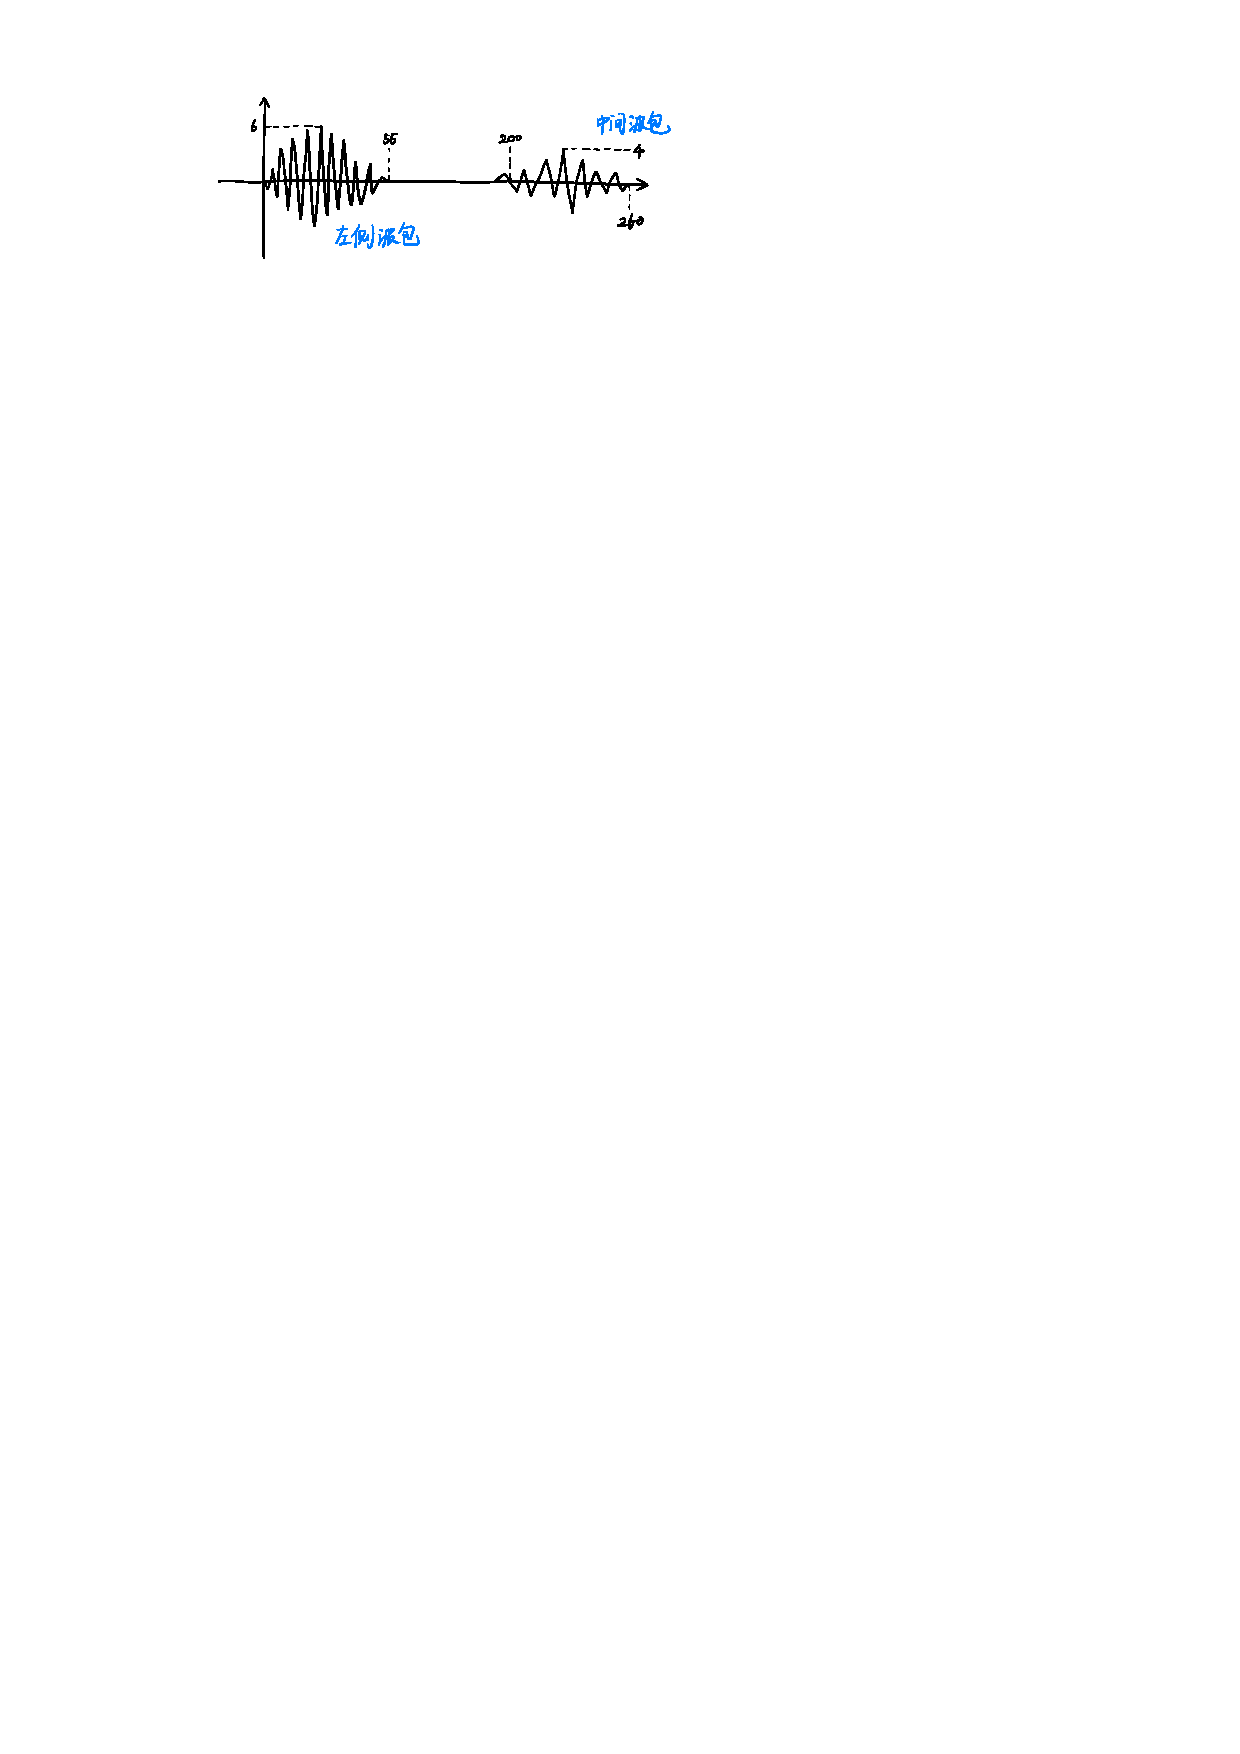
\includegraphics[width=0.8\linewidth]{1.pdf}
	\caption{问题一输出信号示意图}
\end{figure}

\section*{Question 2}
\subsection*{(a)}
易知:
\[
	(1-\frac{5}{4}z^{-1}-\frac{3}{2}z^{-2})Y(z)=(1-z^{-1})X(z)
.\] 
因此差分方程为:
\[
	y[n]-\frac{5}{4}y[n-1]-\frac{3}{2}y[n-2]=x[n]-x[n-1]
.\] 
\subsection*{(b)}
将$y[n]$、$x[n]$ 带入上述差分方程:
\[
    A\cos(\omega n+\phi)
	-
	\frac{5}{4}A\cos(\omega n+\phi-\frac{\pi}{2})
	-
	\frac{3}{2}A\cos(\omega n+\phi-\pi)
	=
	\cos(\omega n)
	-
	\cos(\omega n-\frac{\pi}{2})
.\] 
进而
\[
	\LHS=\frac{5\sqrt{5}}{4}\cos(\omega n+\phi+\atan\frac{1}{2})
	\qand
	\RHS=\sqrt{2}\cos(\omega n+\frac{\pi}{4})
.\]
对比系数有:
\[
	A=\frac{4\sqrt{10}}{25},\ \phi=\frac{\pi}{4}-\atan\frac{1}{2}
.\] 
\section*{Question 3}
(本题求导过程誊写到TeX上过于繁琐,故略去)
\subsection*{(a)}
\[
	\phi_a=\atan(\frac{b\sin\omega}{a+b\cos\omega})
	\implies
	\mathrm{grd}=\frac{ab\cos\omega+b^2}{2ab\cos\omega+a^2+b^2}
.\] 
\subsection*{(b)}
令上一问中$a=1,\,b=c$便能推出此问结果
\[
	\phi_b=-\atan(\frac{c\sin\omega}{1+c\cos\omega})
	\implies
	\mathrm{grd}=-\frac{c\cos\omega+c^2}{2c\cos\omega+1+c^2}
.\] 

\subsection*{(c)}
有上两问便可得到:
\[
	\phi_c=\phi_a+\phi_b
	\implies
	\mathrm{grd}=\frac{ab\cos\omega+b^2}{2ab\cos\omega+a^2+b^2}-\frac{c\cos\omega+c^2}{2c\cos\omega+1+c^2}
.\] 
\subsection*{(d)}
应用(b)问两次:
\[
	\mathrm{grd}=-\frac{c\cos\omega+c^2}{2c\cos\omega+1+c^2}-\frac{d\cos\omega+d^2}{2d\cos\omega+1+d^2}
.\] 
\section*{Question 4}
根据单位圆外的零极点分布:
\[
	H_{ap}(z)=\frac{(z-4)(z-\flatfrac{1}{3})}{(z-\flatfrac{1}{4})(z-3)}
.\] 
进而
\[
	H_{\min}(z)=\frac{H(z)}{H_{ap}(z)}=A\times\frac{z-\flatfrac{1}{4}}{(z-\flatfrac{1}{2})(z-\flatfrac{1}{3})}
.\] 
不考虑幅值的$H_{\min}$、$H_{ap}$是唯一的,他们各自的零极点图如下:
\begin{figure}[htpb]
	\centering
	\begin{minipage}[h]{0.46\linewidth}
		\centering
		\begin{tikzpicture}
			\draw[->] (0,-1.5) -- (0,1.5);
			\draw[->] (-1.5,0) -- (5,0);
			\draw (0,0) circle [radius=1];
			\node (a) at (1/5,0){$\times$};
			\draw[dashed] (1/5,0) -- (1.7,1.5) node{$\frac{1}{4}$};
			\node (a) at (3,0){$\times$};
			\node (a) at (3,-0.5){$3$};
			\node (a) at (4,0){$\circ$};
			\node (a) at (4,-0.5){$4$};
			\node (a) at (1/2,0){$\circ$};
			\draw[dashed] (1/2,0) -- (2,-1) node{$\frac{1}{3}$};
		\end{tikzpicture}
		\caption{$H_{ap}$零极点图}
	\end{minipage}
	\begin{minipage}[h]{0.46\linewidth}
		\centering
		\begin{tikzpicture}
			\draw[->] (0,-3) -- (0,3);
			\draw[->] (-3,0) -- (3,0);
			\draw (0,0) circle [radius=2];
			\node (a) at (1/3,0){$\circ$};
			\node (a) at (1/3,0.5){$\frac{1}{4}$};
			\node (a) at (2/3,0){$\times$};
			\node (a) at (2/3,-0.5){$\frac{1}{3}$};
			\node (a) at (1,0){$\times$};
			\node (a) at (1,0.5){$\frac{1}{2}$};
		\end{tikzpicture}
		\caption{$H_{\min}$零极点图}
	\end{minipage}
\end{figure}


\section*{Question 5}
建系解方程即可,设$\abs{OP}=a,\,\abs{OZ}=b$且$D=(x,y)$:
 \[
	 \alpha^2\qty[(x-b)^2+y^2]=(x-a)^2+y^2
.\] 
$y^2=1-x^2$代入上式:
\[
    2(a-\alpha b)x+\alpha^2+\alpha^2b^2-a^2-1=0
.\] 
对于任意的$x$成立:
\[
    \begin{cases}
    	a=\alpha^2 b\\
		\alpha^2+\alpha^2b^2-a^2-1=0
    \end{cases}
.\] 
从而:
\[
    a=\alpha,\ b=\frac{1}{\alpha}\implies ab=1
.\] 
\end{document}

